\documentclass{article}

\usepackage{graphicx}
\usepackage{tikz}
\usepackage{tikzsymbols}
\usetikzlibrary{calc,patterns,shapes.geometric}
\pagestyle{empty}
\usepackage[margin=0pt]{geometry}
\geometry{papersize={14in,12in}}

\def\centerarc[#1](#2)(#3:#4:#5){\draw[#1] ($(#2)+({#5*cos(#3)},{#5*sin(#3)})$) arc (#3:#4:#5);}

\begin{document}
	\begin{figure}
		\centering
		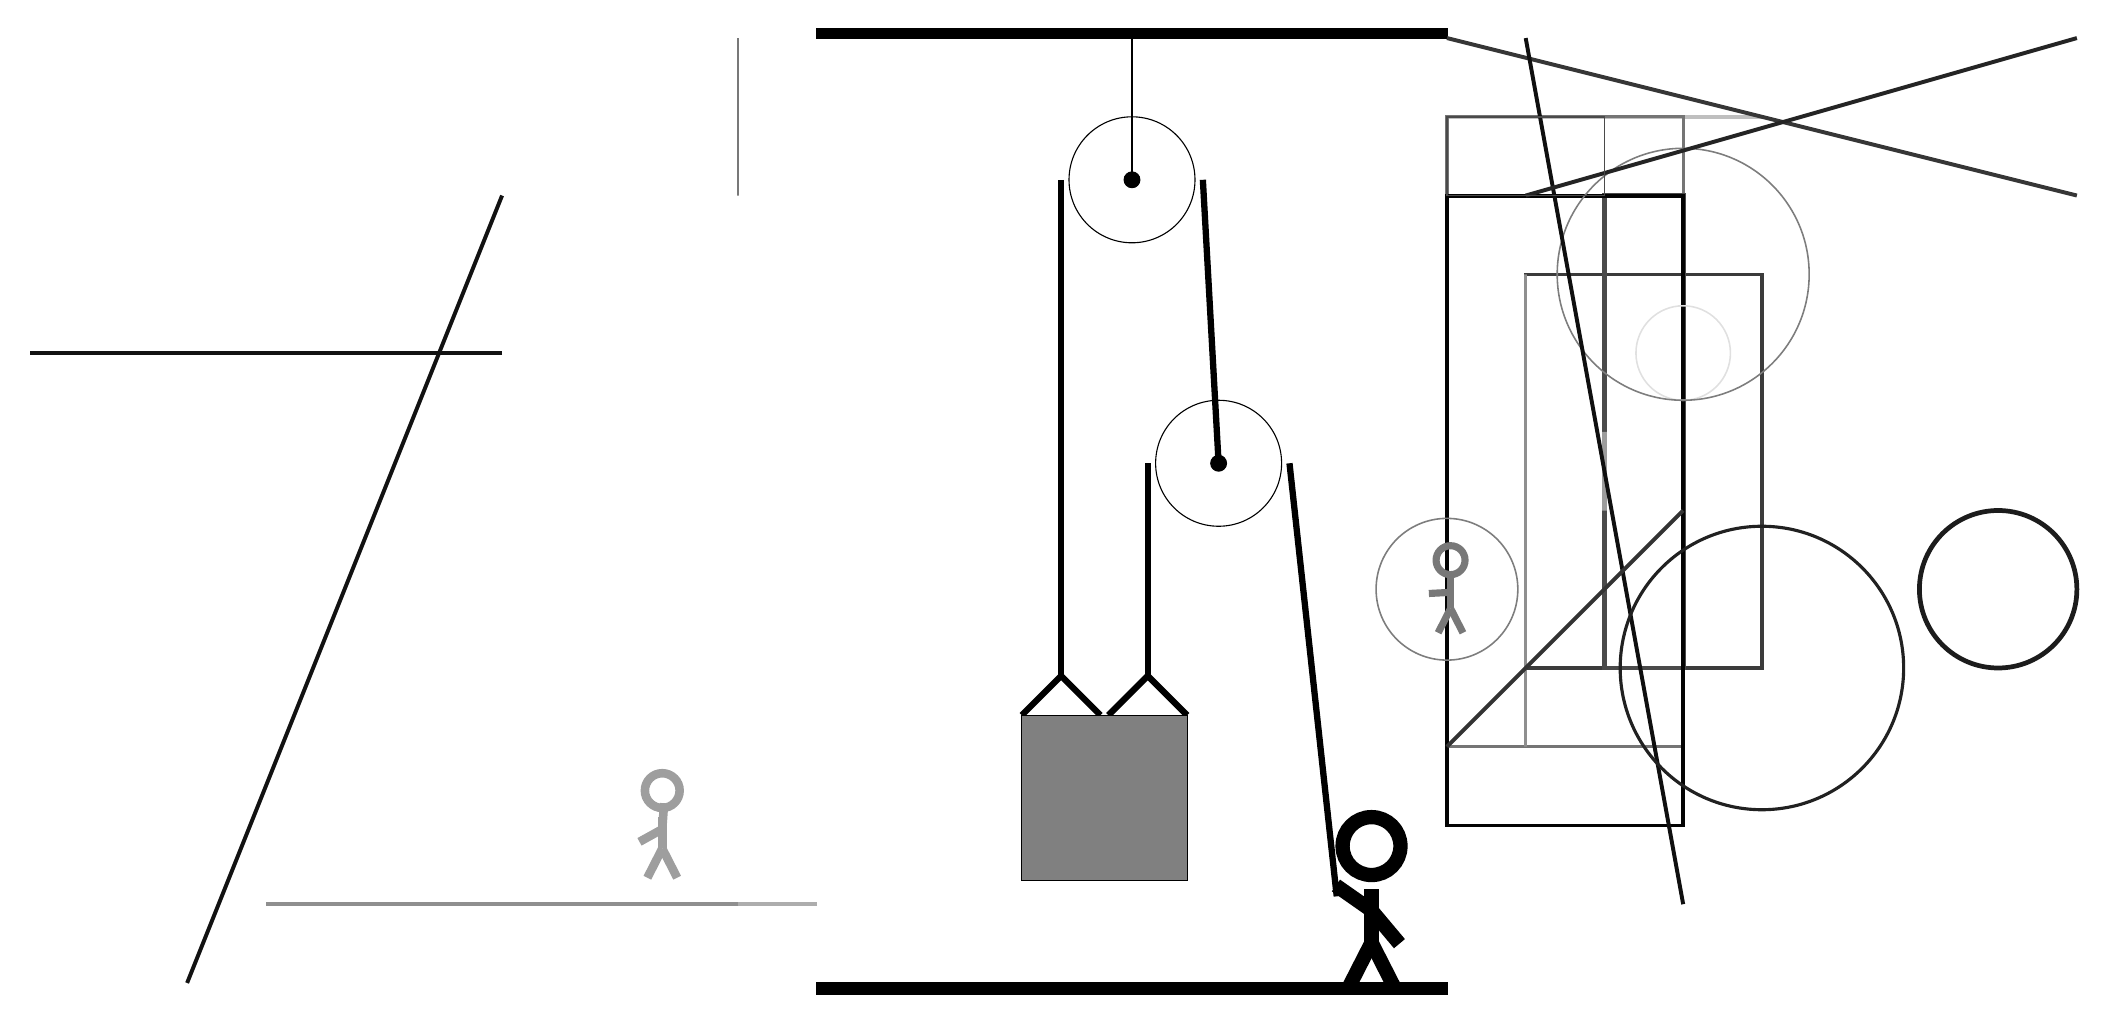
\begin{tikzpicture}
			%%%%% START %%%%%
			
			\draw[fill=black] (-2, 9) rectangle (6, 9.125);
			
			\draw (2, 7.2) circle (0.8);
			\draw[fill=black] (2, 7.2) circle (0.1);
			\draw[thick] (2, 7.2) -- (2, 9);
			
			\draw (3.1, 3.6) circle (0.8);
			\draw[fill=black] (3.1, 3.6) circle (0.1);
			
			\draw [line width=0.7mm, color=black!58](11, 4) circle (0.0);
			
			\draw [line width=0.7mm, color=black!100](-4, -1) circle (0.0);
			\draw[line width=0.3mm, color=black!53] (-3, 9) rectangle (-3, 7);
			\draw[line width=0.4mm, color=black!77] (7, 1) rectangle (10, 6);
			\draw[line width=0.5mm, color=black!25] (6, 8) rectangle (10, 8);
			\draw[line width=0.4mm, color=black!54] (6, 8) rectangle (9, 0);
			\draw[line width=0.5mm, color=black!32](-2, -2) -- (-7, -2);
			\draw[line width=0.5mm, color=black!93](-6, 7) -- (-10, -3);
			\draw [line width=0.4mm, color=black!62](-2, 0) circle (0.0);
			\draw[line width=0.6mm, color=black!71] (8, 1) rectangle (9, 7);
			\draw[line width=0.5mm, color=black!99] (6, -1) rectangle (9, 7);
			
			\node[line width=0.3mm, color=black!53] at (6, 2) {\Strichmaxerl[5][3][90]};
			\draw [line width=0.2mm, color=black!51](6, 2) circle (0.9);
			
			\draw [line width=0.2mm, color=black!12](9, 5) circle (0.6);
			\draw[line width=0.5mm, color=black!79](6, 9) -- (14, 7);
			\draw[line width=0.5mm, color=black!93](-6, 5) -- (-12, 5);
			\draw[line width=0.4mm, color=black!44] (7, 6) rectangle (7, 0);
			\draw[line width=0.7mm, color=black!39] (8, 3) rectangle (8, 4);
			\node[line width=0.2mm, color=black!38] at (-4, -1) {\Strichmaxerl[6][29][86]};
			
			\draw [line width=0.2mm, color=black!51](9, 6) circle (1.6);
			\draw[line width=0.5mm, color=black!94](7, 9) -- (9, -2);
			\draw [line width=0.4mm, color=black!87](10, 1) circle (1.8);
			\draw[line width=0.5mm, color=black!86](7, 7) -- (14, 9);
			\draw[line width=0.5mm, color=black!80](9, 3) -- (6, 0);
			\draw[line width=0.2mm, color=black!71] (8, 8) rectangle (6, 7);
			
			\draw[line width=0.5mm, color=black!44](-3, -2) -- (-9, -2);
			\draw [line width=0.6mm, color=black!89](13, 2) circle (1.0);
			
			\draw[line width = 0.8mm]  (0.6, 0.4) -- (1.1, 0.9) -- (1.6, 0.4);
			\draw[line width = 0.8mm]  (1.7, 0.4) -- (2.2, 0.9) -- (2.7, 0.4);
			\draw[fill=black!50] (0.6, 0.4) rectangle (2.7, -1.7);
			
			\draw[line width = 0.8mm] (1.1, 7.2) -- (1.1, 0.9);
			\centerarc[line width = 0.8mm](2, 7.2)(0:180:0.9);
			\draw[line width = 0.8mm] (2.9, 7.2) -- (3.1, 3.6);
			\draw[line width = 0.8mm] (2.2, 3.6) -- (2.2, 0.9);
			\centerarc[line width = 0.8mm](3.1, 3.6)(0:180:0.9);
			\draw[line width = 0.8mm] (4.0, 3.6) -- (4.6, -1.9);
			
			\node at (5, -2) {\Strichmaxerl[10][-35][-50]};
			
			\draw[fill=black] (-2, -3) rectangle (6, -3.15);
			
			%%%%% END %%%%%
		\end{tikzpicture}
	\end{figure}	
\end{document}